\documentclass[12pt,a4paper]{report}

% ─── Packages ───────────────────────────────────────────────
\usepackage[utf8]{inputenc}
\usepackage[T1]{fontenc}
\usepackage[french,english]{babel}
%\usepackage{times}
\usepackage{graphicx}
\usepackage{hyperref}
\usepackage{geometry}
\usepackage{setspace}
%\usepackage{caption}
\usepackage{float}
\usepackage{longtable}
\usepackage{array}
\usepackage{xcolor}
\usepackage{listings}
\usepackage{fancyhdr}

% ─── Page Layout ────────────────────────────────────────────
\geometry{left=2.5cm, right=2.5cm, top=2.5cm, bottom=2.5cm}
\onehalfspacing

% ─── Header/Footer ──────────────────────────────────────────
\pagestyle{fancy}
\fancyhf{}
\fancyhead[L]{\leftmark}
\fancyhead[R]{\thepage}
\renewcommand{\headrulewidth}{0.4pt}

% ─── Table of Contents ──────────────────────────────────────

% ─── Code Style ─────────────────────────────────────────────
\lstdefinestyle{custom}{
  basicstyle=\footnotesize\ttfamily,
  breaklines=true,
  frame=single,
  numbers=left,
  numberstyle=\tiny,
  backgroundcolor=\color{gray!10}
}

% ─── Document Info ──────────────────────────────────────────
\title{Observatory Analysis\\\large Adaptive Digital Observatory for ISET Tozeur}
\author{Noureddine Jabnouni}
\date{2025/2026}

\begin{document}

% ─── Cover Page ─────────────────────────────────────────────
\begin{titlepage}
\begin{center}
\vspace*{1cm}

\includegraphics[width=0.3\textwidth]{res/iset_logo.png}\\[1cm]

\textsc{\Large Ministry of Higher Education\\and Scientific Research}\\[0.3cm]
\textsc{\Large Directorate General of Technological Studies}\\[0.3cm]
\textsc{\Large Higher Institute of Technological Studies of Tozeur}\\[1.5cm]

\rule{\linewidth}{0.5mm}\\[0.4cm]
{\huge\bfseries Observatory Analysis\\[0.5cm]
\large Adaptive Digital Observatory ---\\Data Management \& AI Analytics Platform}\\[0.4cm]
\rule{\linewidth}{0.5mm}\\[1.5cm]

\textsc{\Large Graduation Project Report}\\[0.5cm]
\textsc{\Large Presented for the degree of\\Licence in Information Technology}\\[1.5cm]

\vfill

\begin{tabular}{lr}
\textbf{Prepared by:} & Noureddine \textsc{Jabnouni}\\
\textbf{Supervised by:} & Mr.~Soufiene \textsc{Ben Mahmoud}\\
\textbf{Host Organization:} & ISET Tozeur\\
\textbf{Academic Year:} & 2025/2026\\
\end{tabular}

\vspace{1cm}
\end{center}
\end{titlepage}

% ─── Signature Page ─────────────────────────────────────────
\newpage
\thispagestyle{empty}
\vspace*{4cm}
\begin{center}
{\Large\bfseries Signatures}
\end{center}
\vspace{1cm}

\begin{center}
\begin{tabular}{p{5cm}p{5cm}p{5cm}}
\rule{5cm}{0.4pt} & \rule{5cm}{0.4pt} & \rule{5cm}{0.4pt} \\
ISET Supervisor & Company Supervisor & Student \\
Mr.~Soufiene Ben Mahmoud & \hspace{3cm} & Noureddine Jabnouni \\
\end{tabular}
\end{center}

% ─── Résumé / Abstract ─────────────────────────────────────
\newpage
\thispagestyle{empty}
\begin{center}
{\Large\bfseries Résumé}
\end{center}
\vspace{0.5cm}

Ce projet présente le développement d'\textbf{Observatory Analysis}, une plateforme web modulaire de gestion, d'analyse et de visualisation de données destinée à l'Institut Supérieur des Études Technologiques (ISET) de Tozeur. La plateforme permet aux administrateurs d'importer des fichiers CSV et Excel, de créer dynamiquement des tables PostgreSQL, d'explorer les données, de construire des graphiques interactifs, de composer des tableaux de bord, d'utiliser l'intelligence artificielle pour des requêtes en langage naturel, de générer des enquêtes et des rapports, et de gérer les utilisateurs avec un contrôle d'accès basé sur les rôles (RBAC).

L'architecture technique repose sur React 19 et TypeScript pour le frontend, Node.js avec Express et TypeScript pour le backend, et PostgreSQL 15 comme système de gestion de base de données. L'ensemble est conteneurisé avec Docker et Docker Compose. L'intégration de l'IA est assurée par l'API Groq avec le modèle \textit{qwen/qwen3-32b} pour les fonctionnalités de requêtes en langage naturel, la génération d'enquêtes et la production de rapports.

\vspace{0.3cm}
\textbf{Mots-clés :} Analyse de données, Visualisation, Intelligence Artificielle, React, Node.js, PostgreSQL, Dashboard, RBAC, ISET Tozeur.

\vspace{1cm}
\begin{center}
{\Large\bfseries Abstract}
\end{center}
\vspace{0.5cm}

This project presents the development of \textbf{Observatory Analysis}, a modular web platform for data management, analysis, and visualization designed for the Higher Institute of Technological Studies (ISET) of Tozeur. The platform enables administrators to import CSV and Excel files, dynamically create PostgreSQL tables, explore data, build interactive charts, compose dashboards, leverage artificial intelligence for natural language queries, generate surveys and reports, and manage users with role-based access control (RBAC).

The technical architecture uses React 19 with TypeScript for the frontend, Node.js with Express and TypeScript for the backend, and PostgreSQL 15 as the database management system. The entire stack is containerized with Docker and Docker Compose. AI integration is powered by the Groq API using the \textit{qwen/qwen3-32b} model for natural language querying, survey generation, and report production.

\vspace{0.3cm}
\textbf{Keywords:} Data Analysis, Visualization, Artificial Intelligence, React, Node.js, PostgreSQL, Dashboard, RBAC, ISET Tozeur.

% ─── Acknowledgments ───────────────────────────────────────
\newpage
\thispagestyle{empty}
\begin{center}
{\Large\bfseries Acknowledgments}
\end{center}
\vspace{0.5cm}

I would like to express my sincere gratitude to all those who contributed to the successful completion of this graduation project.

First and foremost, I thank my supervisor, Mr.~Soufiene Ben Mahmoud, for his invaluable guidance, support, and insightful feedback throughout this project. His expertise and encouragement have been instrumental in shaping this work.

I am grateful to the faculty and staff of ISET Tozeur for providing me with the knowledge and skills necessary to undertake this endeavor.

Special thanks to my family for their unwavering support and encouragement throughout my academic journey.

Finally, I thank all my friends and colleagues who have supported me along the way.

% ─── Dedication ─────────────────────────────────────────────
\newpage
\thispagestyle{empty}
\begin{center}
{\Large\bfseries Dedication}
\end{center}
\vspace{1cm}

To my dear parents,\\
No dedication could express my profound love, immense gratitude, and greatest respect, as I will never forget the tenderness and devoted love with which they have surrounded me since childhood.

To my family,\\
For the encouragement and kindness they have given me, I express my deep gratitude and great respect.

To my supervisor,\\
For exceptional supervision, enlightened advice, and constant support throughout this project.

To all my professors,\\
Who taught me throughout my studies and ensured my training under the best conditions.

To all my friends,\\
Who have always encouraged me, to whom I wish even more success.

% ─── Table of Contents ─────────────────────────────────────
\newpage
\tableofcontents

% ─── List of Figures ───────────────────────────────────────
\newpage
\listoffigures

% ─── List of Tables ─────────────────────────────────────────
\newpage
\listoftables

% ─── List of Abbreviations ─────────────────────────────────
\newpage
\begin{center}
{\Large\bfseries List of Abbreviations}
\end{center}
\vspace{0.5cm}

\begin{table}[H]\begin{tabular}{p{0.2\textwidth} p{0.75\textwidth}}
\textbf{API} & Application Programming Interface \\
\textbf{CRUD} & Create, Read, Update, Delete \\
\textbf{CSV} & Comma-Separated Values \\
\textbf{Docker} & Containerization Platform \\
\textbf{GPA} & Grade Point Average \\
\textbf{Groq} & AI Inference Platform \\
\textbf{HTTP} & Hypertext Transfer Protocol \\
\textbf{ISET} & Institut Supérieur des Études Technologiques \\
\textbf{JSON} & JavaScript Object Notation \\
\textbf{JWT} & JSON Web Token \\
\textbf{KPI} & Key Performance Indicator \\
\textbf{LLM} & Large Language Model \\
\textbf{NL} & Natural Language \\
\textbf{RBAC} & Role-Based Access Control \\
\textbf{REST} & Representational State Transfer \\
\textbf{SPA} & Single Page Application \\
\textbf{SQL} & Structured Query Language \\
\end{tabular}\end{table}

% ─── Glossary ──────────────────────────────────────────────
\newpage
\begin{center}
{\Large\bfseries Glossary}
\end{center}
\vspace{0.5cm}

\begin{table}[H]\begin{tabular}{p{0.2\textwidth} p{0.75\textwidth}}
\textbf{Chart.js} & JavaScript library for creating interactive charts \\
\textbf{Dashboard} & Visual display of key data points and charts \\
\textbf{Dataset} & Collection of data imported into the system \\
\textbf{Dynamic Table} & Auto-created PostgreSQL table from imported data \\
\textbf{Groq} & Fast AI inference platform for LLM queries \\
\textbf{Middleware} & Software layer that handles request processing \\
\textbf{Migration} & Automated database schema update \\
\textbf{RBAC} & Security approach restricting system access to authorized users \\
\end{tabular}\end{table}

% ══════════════════════════════════════════════════════════════
% GENERAL INTRODUCTION
% ══════════════════════════════════════════════════════════════
\chapter*{General Introduction}
\addcontentsline{toc}{chapter}{General Introduction}

In the rapidly evolving landscape of higher education, data has become an invaluable asset for institutional decision-making, quality assurance, and strategic planning. Educational institutions collect vast amounts of data ranging from student academic records and course outcomes to alumni employment statistics and survey feedback. However, this data often remains underutilized, trapped in isolated spreadsheets and disparate systems that do not communicate with each other.

The Higher Institute of Technological Studies (ISET) of Tozeur, like many academic institutions, faces the challenge of centralizing, analyzing, and visualizing its institutional data effectively. The need for a unified platform that can import heterogeneous data sources, provide intuitive exploration tools, generate actionable insights, and support decision-making through interactive visualizations became increasingly apparent.

This project, \textbf{Observatory Analysis}, addresses this challenge by developing an adaptive digital observatory platform. The system provides a comprehensive suite of tools including:
\begin{itemize}
    \item A schema-agnostic data import engine that accepts CSV and Excel files of any structure
    \item An interactive database explorer with full CRUD capabilities on dynamic tables
    \item A versatile chart builder supporting ten chart types
    \item A drag-and-drop dashboard composer with PDF export
    \item An AI-powered natural language query interface for data analysis
    \item A survey generation and management system with AI assistance
    \item A role-based access control system for granular permission management
    \item A client portal for students, alumni, and teachers
\end{itemize}

The platform was developed using modern web technologies including React 19, TypeScript, Node.js, Express, and PostgreSQL 15. The AI capabilities are powered by Groq's API using the \textit{qwen/qwen3-32b} model. The entire application is containerized with Docker for consistent deployment across environments.

This report is organized into six chapters. \textbf{Chapter 1} presents the general framework of the project, including the host organization, problem statement, objectives, methodology, and working environment. \textbf{Chapter 2} covers the study and analysis phase, including the product backlog, sprint planning, and system design. \textbf{Chapters 3 through 6} detail the realization of each sprint, showcasing the implemented features through diagrams and screenshots. The report concludes with a general conclusion summarizing the achievements, limitations, and future perspectives.

% ══════════════════════════════════════════════════════════════
% CHAPTER 1: GENERAL FRAMEWORK
% ══════════════════════════════════════════════════════════════
\chapter{General Framework of the Project}

\section{Presentation of the Host Organization}

\subsection{ISET Tozeur}

The Higher Institute of Technological Studies (ISET) of Tozeur is a public institution of higher education under the supervision of the Ministry of Higher Education and Scientific Research of Tunisia. Established to provide quality technological education, ISET Tozeur offers Bachelor's degrees (License) in various fields including Information Technology, Electrical Engineering, Management, and Civil Engineering.

The institute is committed to:
\begin{itemize}
    \item Training highly qualified technicians and professionals
    \item Fostering innovation and research in applied technologies
    \item Strengthening partnerships with the socio-economic sector
    \item Contributing to regional development in the Tozeur region
\end{itemize}

\subsection{Organizational Structure}

The host organization operates under the direction of a General Director, supported by:
\begin{itemize}
    \item The Department of Academic Affairs
    \item The Department of Student Affairs
    \item The Department of Research and Innovation
    \item Various academic departments (Informatique, Electrique, Gestion, Génie Civil)
    \item The Information Systems Division
\end{itemize}

\section{Context and Problem Statement}

\subsection{Current Situation}

ISET Tozeur currently manages its institutional data through a combination of:
\begin{itemize}
    \item Manual spreadsheets (Excel) for student records and grades
    \item Paper-based surveys for alumni tracking
    \item Disconnected databases for different administrative functions
    \item Manual report generation processes
\end{itemize}

\subsection{Identified Problems}

The analysis of the current situation revealed several challenges:
\begin{enumerate}
    \item \textbf{Data Fragmentation:} Institutional data is scattered across multiple files and formats, making it difficult to obtain a unified view.
    \item \textbf{Limited Analysis Capabilities:} Without proper tools, extracting insights from data requires significant manual effort and technical expertise.
    \item \textbf{Lack of Visualization:} Decision-makers lack interactive visualizations to understand trends and patterns in the data.
    \item \textbf{Absence of AI Integration:} Natural language querying and automated report generation are not available.
    \item \textbf{No Centralized Client Portal:} Students, alumni, and teachers lack a unified portal to access their information and provide feedback.
    \item \textbf{Inefficient Survey Management:} Survey creation, distribution, and analysis are manual and time-consuming processes.
\end{enumerate}

\section{Objectives}

\subsection{General Objective}

The main objective of this project is to design and develop a web-based adaptive digital observatory platform that centralizes, analyzes, and visualizes institutional data for ISET Tozeur.

\subsection{Specific Objectives}

\begin{enumerate}
    \item Design a modular and scalable system architecture
    \item Implement a schema-agnostic data import engine for CSV and Excel files
    \item Develop an interactive data exploration and table management interface
    \item Create a versatile chart builder supporting multiple visualization types
    \item Build a drag-and-drop dashboard composer with PDF export capabilities
    \item Integrate AI-powered natural language querying using Groq's LLM
    \item Implement an AI-assisted survey generation and management system
    \item Develop a role-based access control system for granular permission management
    \item Create a client portal for students, alumni, and teachers
    \item Implement a comprehensive theme and internationalization system
\end{enumerate}

\section{Methodology}

\subsection{Agile Methodology}

The project was developed using the \textbf{Scrum} agile framework, which emphasizes iterative development, collaboration, and continuous improvement. Scrum was chosen for the following reasons:
\begin{itemize}
    \item \textbf{Flexibility:} Allows adaptation to changing requirements
    \item \textbf{Communication:} Encourages regular interaction between team members
    \item \textbf{Rapid Delivery:} Delivers functional increments through sprints
    \item \textbf{Quality:} Continuous testing and integration ensure high quality
\end{itemize}

\subsection{Scrum Roles}

\begin{table}[H]
\centering
\begin{tabular}{|l|l|}
\hline
\textbf{Role} & \textbf{Responsible} \\
\hline
Product Owner & Mr.~Soufiene Ben Mahmoud \\
Scrum Master & Noureddine Jabnouni \\
Development Team & Noureddine Jabnouni \\
\hline
\end{tabular}
\caption{Scrum Roles}
\end{table}

\subsection{Sprint Planning}

The project was organized into four 4-week sprints, each focusing on the implementation of a specific set of features:

\begin{table}[H]
\centering
\begin{tabular}{|l|l|p{8cm}|}
\hline
\textbf{Sprint} & \textbf{Duration} & \textbf{Main Features} \\
\hline
Sprint 1 & 4 weeks & Authentication, RBAC, Data Import, Database Explorer, Table Editor \\
Sprint 2 & 4 weeks & Chart Builder, Dashboard Canvas, Foreign Keys, Saved Queries \\
Sprint 3 & 4 weeks & AI Analysis, Survey Generator, Reports, Client Portal \\
Sprint 4 & 4 weeks & Settings, Themes, Internationalization, Public Access, Polish \\
\hline
\end{tabular}
\caption{Sprint Planning}
\end{table}

\section{Working Environment}

\subsection{Software Environment}

\begin{table}[H]
\centering
\begin{tabular}{|l|l|}
\hline
\textbf{Tool} & \textbf{Purpose} \\
\hline
Visual Studio Code & Code editor \\
Docker \& Docker Compose & Container orchestration \\
PostgreSQL 15 & Database management \\
Git \& GitHub & Version control \\
Postman & API testing \\
\hline
\end{tabular}
\caption{Software Tools}
\end{table}

\subsection{Technologies Used}

\subsubsection{Frontend Technologies}

\begin{table}[H]
\centering
\begin{tabular}{|l|l|}
\hline
\textbf{Technology} & \textbf{Purpose} \\
\hline
React 19 & UI framework \\
TypeScript 5 & Type-safe JavaScript \\
Vite & Build tool and development server \\
Ant Design 6 & UI component library \\
Chart.js 4 & Chart rendering \\
React Router DOM 7 & Client-side routing \\
i18next & Internationalization \\
Axios & HTTP client \\
jsPDF & PDF export \\
PapaParse & CSV parsing \\
\hline
\end{tabular}
\caption{Frontend Technologies}
\end{table}

\subsubsection{Backend Technologies}

\begin{table}[H]
\centering
\begin{tabular}{|l|l|}
\hline
\textbf{Technology} & \textbf{Purpose} \\
\hline
Node.js 20 & JavaScript runtime \\
Express 5 & Web framework \\
TypeScript 5 & Type safety \\
PostgreSQL 15 & Database \\
jsonwebtoken & JWT authentication \\
bcryptjs & Password hashing \\
Groq SDK & AI integration \\
Multer & File upload handling \\
ExcelJS & Excel file parsing \\
\hline
\end{tabular}
\caption{Backend Technologies}
\end{table}

\subsubsection{Infrastructure}

\begin{table}[H]
\centering
\begin{tabular}{|l|l|}
\hline
\textbf{Technology} & \textbf{Purpose} \\
\hline
Docker \& Docker Compose & Containerization \\
Railway & Backend hosting \\
Vercel & Frontend hosting \\
Groq AI & LLM provider \\
\hline
\end{tabular}
\caption{Infrastructure Technologies}
\end{table}

\subsection{Hardware Environment}

\begin{table}[H]
\centering
\begin{tabular}{|l|l|}
\hline
\textbf{Component} & \textbf{Specification} \\
\hline
Processor & Ryzen 5 3600 \\
RAM & 16 GB \\
Storage & 512 GB SSD \\
Operating System & Linux \\
\hline
\end{tabular}
\caption{Development Hardware Specifications}
\end{table}

% ══════════════════════════════════════════════════════════════
% CHAPTER 2: SPRINT 0 - STUDY AND ANALYSIS
% ══════════════════════════════════════════════════════════════
\chapter{Sprint 0: Study and Analysis}

\section{Introduction}

Before embarking on the implementation phase, a thorough study and analysis of the project was conducted. This chapter presents the product backlog, sprint planning, system architecture, and design diagrams that served as the foundation for the development process.

\section{Product Backlog}

The product backlog is a prioritized list of features and functionalities to be developed throughout the project. Each item is described as a user story following the format: "As a [role], I want to [action], so that [benefit]."

\begin{table}[H]\begin{tabular}{|p{0.5cm}|p{2.5cm}|p{4cm}|p{1cm}|p{1.5cm}|}
\hline
\textbf{\#} & \textbf{Role} & \textbf{User Story} & \textbf{Priority} & \textbf{Sprint} \\
\hline

\hline
\textbf{\#} & \textbf{Role} & \textbf{User Story} & \textbf{Priority} & \textbf{Sprint} \\
\hline

1 & Visitor & View landing page to discover the platform & High & 1 \\
2 & Visitor & Create an account to access platform features & High & 1 \\
3 & User & Log in to securely access my account & High & 1 \\
4 & User & Manage profile to keep information up to date & Medium & 1 \\
5 & Admin & Import CSV/Excel files to centralize data & High & 1 \\
6 & Admin & Explore and manage imported data tables & High & 1 \\
7 & Admin & Create charts from data to visualize trends & High & 2 \\
8 & Admin & Build dashboards to display key metrics & High & 2 \\
9 & Admin & Manage foreign keys to link data tables & Medium & 2 \\
10 & Admin & Save and execute SQL queries & Medium & 2 \\
11 & Admin & Query data using natural language via AI & High & 3 \\
12 & Admin & Generate surveys to collect feedback & High & 3 \\
13 & Admin & Generate AI performance reports & High & 3 \\
14 & Admin & Manage users and roles with RBAC & High & 4 \\
15 & Admin & Manage client accounts & High & 4 \\
16 & Client & View published dashboards & High & 3 \\
17 & Client & Take surveys and provide feedback & High & 3 \\
18 & Client & View performance reports & Medium & 3 \\
19 & Public & View public dashboards without login & Medium & 4 \\
20 & Public & Submit survey responses anonymously & Medium & 4 \\
\hline
\caption{Product Backlog}
\end{tabular}\end{table}

\section{System Architecture}

The application follows a three-tier architecture pattern comprising the presentation layer (React frontend), the application layer (Express backend), and the data layer (PostgreSQL database). The entire stack is containerized using Docker.

\begin{figure}[H]
\centering
\includegraphics[width=\textwidth]{res/diagram-system_architecture.png}
\caption{System Architecture Diagram}
\end{figure}

\subsection{Architecture Components}

\begin{enumerate}
    \item \textbf{Presentation Layer:} A React 19 single-page application (SPA) built with TypeScript and Vite. The UI is powered by Ant Design components with support for theming and internationalization.
    \item \textbf{Application Layer:} A Node.js Express API server written in TypeScript. It provides RESTful endpoints for all platform operations and integrates with Groq AI for natural language processing.
    \item \textbf{Data Layer:} PostgreSQL 15 relational database that stores both system metadata (users, roles, permissions) and dynamic data tables created from imported files.
\end{enumerate}

\section{Use Case Diagrams}

\subsection{Admin Use Cases}

The administrator has access to the full range of platform features, including data management, analytics, user administration, and system configuration.

\begin{figure}[H]
\centering
\includegraphics[width=\textwidth]{res/diagram-use_case_admin.png}
\caption{Use Case Diagram --- Administrator}
\end{figure}

\subsection{Client and Public Use Cases}

Clients (students, alumni, teachers) can access published content, take surveys, and view reports. Guest users can access public dashboards and submit survey responses.

\begin{figure}[H]
\centering
\includegraphics[width=\textwidth]{res/diagram-use_case_client.png}
\caption{Use Case Diagram --- Client and Public Users}
\end{figure}

\section{Sequence Diagrams}

\subsection{Login Sequence}

The authentication process involves credential validation, JWT token generation, and session management on the frontend.

\begin{figure}[H]
\centering
\includegraphics[width=0.9\textwidth]{res/diagram-sequence_login.png}
\caption{Sequence Diagram --- User Login}
\end{figure}

\subsection{Data Import Sequence}

The data import workflow involves file upload, parsing, column mapping, and dynamic table creation with bulk data insertion.

\begin{figure}[H]
\centering
\includegraphics[width=\textwidth]{res/diagram-sequence_data_import.png}
\caption{Sequence Diagram --- Data Import}
\end{figure}

\subsection{AI Query Sequence}

The AI-powered natural language query process converts user questions into SQL queries, executes them against the database, and returns structured results with insights.

\begin{figure}[H]
\centering
\includegraphics[width=0.9\textwidth]{res/diagram-sequence_ai_query.png}
\caption{Sequence Diagram --- AI Natural Language Query}
\end{figure}

\section{Class Diagram}

The class diagram illustrates the database schema and relationships between the main entities of the system.

\begin{figure}[H]
\centering
\includegraphics[width=\textwidth]{res/diagram-class_diagram.png}
\caption{Class Diagram --- Database Schema}
\end{figure}

The diagram shows the key entities and their relationships:
\begin{itemize}
    \item \textbf{User} and \textbf{Role} with many-to-many relationship through \texttt{user\_roles}
    \item \textbf{Role} and \textbf{Permission} with many-to-many relationship through \texttt{role\_permissions}
    \item \textbf{Dataset} linked to \textbf{User} (uploader) and to \textbf{Chart} (data source)
    \item \textbf{Dashboard} containing multiple \textbf{Charts}
    \item \textbf{Survey} collecting responses from \textbf{Clients}
    \item \textbf{Report} associated with \textbf{Client} and \textbf{Dataset}
\end{itemize}

\section{Activity Diagram}

The survey creation and response workflow illustrates the process from defining the survey goal to collecting responses.

\begin{figure}[H]
\centering
\includegraphics[width=0.8\textwidth]{res/diagram-activity_survey.png}
\caption{Activity Diagram --- Survey Creation and Response Workflow}
\end{figure}

\section{Conclusion}

In this chapter, we presented a comprehensive analysis of the project, including the product backlog, system architecture, and various UML diagrams. This analysis provided a solid foundation for the implementation phases that follow. The next chapter presents the realization of Sprint 1, focusing on authentication and data management features.

% ══════════════════════════════════════════════════════════════
% CHAPTER 3: SPRINT 1 - AUTHENTICATION AND DATA MANAGEMENT
% ══════════════════════════════════════════════════════════════
\chapter{Sprint 1: Authentication and Data Management}

\section{Introduction}

The first sprint established the foundational features required by all subsequent sprints: authentication, role-based access control, and data import/management capabilities. These core components ensure that users can securely access the system, that their permissions are properly handled, and that administrators can import and manage institutional data.

\section{Sprint Backlog}

\begin{table}[H]\begin{tabular}{|p{0.5cm}|p{2.5cm}|p{4cm}|p{2.5cm}|}
\hline
\textbf{\#} & \textbf{Feature} & \textbf{User Story} & \textbf{Tasks} \\
\hline

\hline
\textbf{\#} & \textbf{Feature} & \textbf{User Story} & \textbf{Tasks} \\
\hline

1 & Landing Page & As a visitor, I want to view the landing page to discover the platform & Design \& develop landing page with marketing content \\
2 & Registration & As a visitor, I want to create an account to access platform features & Build registration form with validation \\
3 & Authentication & As a user, I want to log in to securely access my account & Implement JWT-based login with bcrypt password hashing \\
4 & Profile & As a user, I want to manage my profile to keep info updated & Build profile page with edit/delete capabilities \\
5 & RBAC & As an admin, I want to manage roles and permissions & Implement role CRUD and permission assignment \\
6 & Data Import & As an admin, I want to import CSV/Excel files & Build upload UI with column mapping wizard \\
7 & Data Explorer & As an admin, I want to browse imported tables & Build database explorer with search and filter \\
8 & Table Editor & As an admin, I want to edit table data & Build inline table editor with CRUD operations \\
\hline
\caption{Sprint 1 Backlog}
\end{tabular}\end{table}

\section{Design}

\subsection{Authentication Flow}

The authentication system uses JSON Web Tokens (JWT) for stateless authentication. The login flow was described in the sequence diagram in Chapter 2. The system supports two login modes:
\begin{itemize}
    \item \textbf{Staff Login:} Email and password for administrators and staff
    \item \textbf{Client Login:} Username and password for students, alumni, and teachers
\end{itemize}

\subsection{Authorization Architecture}

The RBAC system is built on three core concepts:
\begin{enumerate}
    \item \textbf{Users:} Individuals who access the system
    \item \textbf{Roles:} Named collections of permissions (e.g., super\_admin, admin, analyst, viewer)
    \item \textbf{Permissions:} Granular access rights (e.g., users.view, data.import, ai.query)
\end{enumerate}

The authorization middleware checks permissions at the route level, ensuring that only authorized users can access specific features.

\section{Realization}

\subsection{Landing Page}

The landing page serves as the main entry point of the platform, providing an overview of features and guiding users toward authentication.

\begin{figure}[H]
\centering
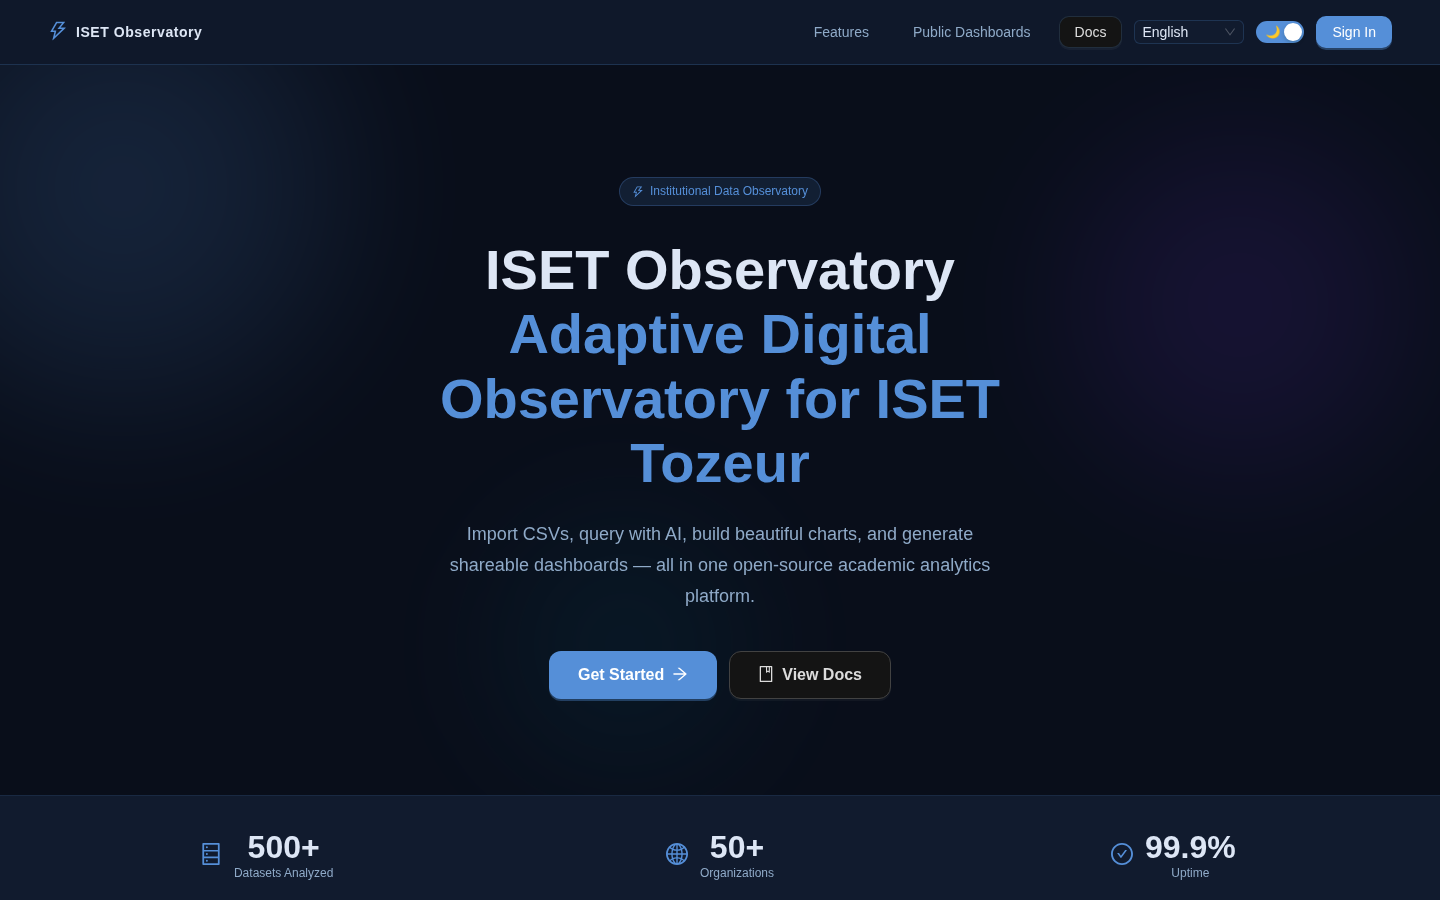
\includegraphics[width=\textwidth]{res/figure-01-landing-page-en.png}
\caption{Landing Page}
\end{figure}

\subsection{Login Page}

The login page provides separate authentication paths for staff members and client users, with form validation and error handling.

\begin{figure}[H]
\centering
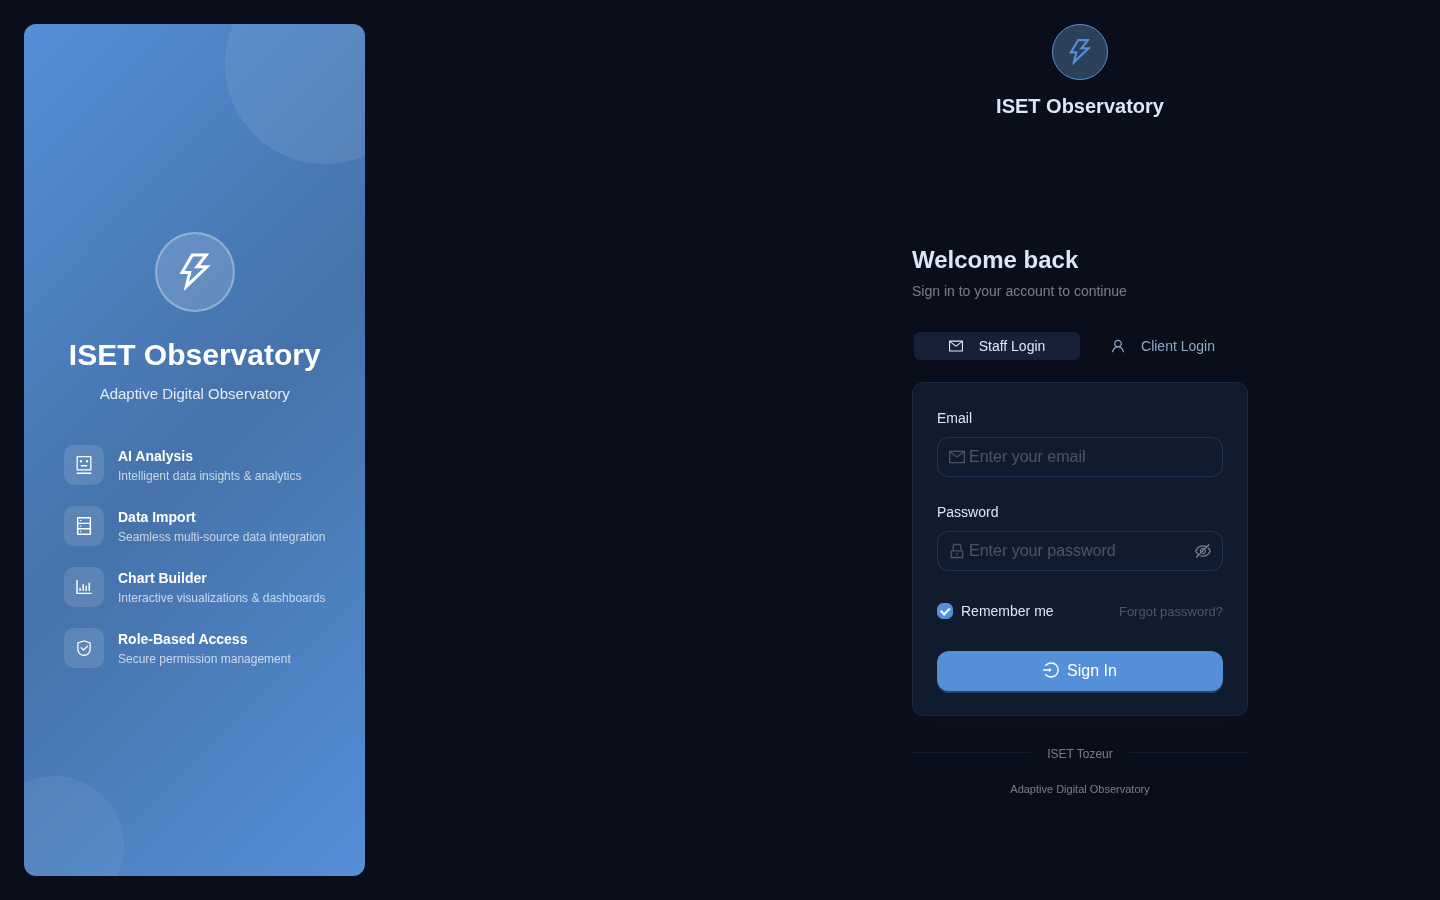
\includegraphics[width=\textwidth]{res/figure-02-login-page-en.png}
\caption{Login Page}
\end{figure}

\subsection{Admin Dashboard}

The admin dashboard provides a centralized view of system statistics, including user counts, dataset metrics, chart counts, and recent activity. Quick action buttons enable rapid access to common tasks.

\begin{figure}[H]
\centering
\includegraphics[width=\textwidth]{res/figure-04-admin-dashboard.png}
\caption{Admin Dashboard}
\end{figure}

\subsection{Data Import Interface}

The data import tool allows administrators to upload CSV or Excel files, preview their content, configure column mappings and types, and import data into dynamically created PostgreSQL tables.

\begin{figure}[H]
\centering
\includegraphics[width=\textwidth]{res/figure-05-data-import-upload.png}
\caption{Data Import Upload Interface}
\end{figure}

\subsection{Database Explorer}

The database explorer displays all imported datasets as interactive cards showing table names, row counts, and import status. Users can search, filter, and sort through their datasets.

\begin{figure}[H]
\centering
\includegraphics[width=\textwidth]{res/figure-06-database-explorer.png}
\caption{Database Explorer}
\end{figure}

\subsection{Table Editor}

The table editor provides a full-featured interface for viewing and manipulating imported data. It supports inline editing, row insertion and deletion, column management, data profiling, and export to CSV or JSON formats.

\begin{figure}[H]
\centering
\includegraphics[width=\textwidth]{res/figure-07-table-editor.png}
\caption{Table Editor Interface}
\end{figure}

\begin{figure}[H]
\centering
\includegraphics[width=\textwidth]{res/figure-33-table-editor-data.png}
\caption{Table Editor --- Data View with Profiling}
\end{figure}

\subsection{Foreign Key Manager}

The foreign key management tool allows administrators to define logical relationships between tables. It supports manual linking, auto-detection, and AI-suggested relationships.

\begin{figure}[H]
\centering
\includegraphics[width=\textwidth]{res/figure-08-foreign-keys-manager.png}
\caption{Foreign Key Manager}
\end{figure}

\subsection{Saved Queries}

The saved queries feature enables users to store, execute, and share SQL queries. Results are displayed in a paginated table and can be exported.

\begin{figure}[H]
\centering
\includegraphics[width=\textwidth]{res/figure-09-saved-queries.png}
\caption{Saved Queries Interface}
\end{figure}

\section{Conclusion}

During this sprint, we successfully implemented the foundational features of the platform: authentication with JWT, role-based access control, data import from CSV and Excel files, database exploration, table editing, foreign key management, and saved queries. These features provide a solid base for the analytics and AI capabilities that subsequent sprints will introduce.

% ══════════════════════════════════════════════════════════════
% CHAPTER 4: SPRINT 2 - ANALYTICS AND VISUALIZATION
% ══════════════════════════════════════════════════════════════
\chapter{Sprint 2: Analytics and Visualization}

\section{Introduction}

After establishing the data management foundation in Sprint 1, this sprint focuses on transforming imported data into meaningful visualizations. The chart builder, dashboard canvas, and supporting features enable administrators to create interactive visual representations of their institutional data.

\section{Sprint Backlog}

\begin{table}[H]\begin{tabular}{|p{0.5cm}|p{2.5cm}|p{4cm}|p{2.5cm}|}
\hline
\textbf{\#} & \textbf{Feature} & \textbf{User Story} & \textbf{Tasks} \\
\hline

\hline
\textbf{\#} & \textbf{Feature} & \textbf{User Story} & \textbf{Tasks} \\
\hline

1 & Chart Builder & As an admin, I want to create charts from imported data & Build chart creation UI with 10 chart types \\
2 & Chart Library & As an admin, I want to manage saved charts & Implement chart CRUD with gallery view \\
3 & Dashboard Canvas & As an admin, I want to compose dashboards with charts & Build drag-and-drop dashboard layout \\
4 & PDF Export & As an admin, I want to export dashboards as PDF & Implement PDF generation with jsPDF \\
5 & Dashboard Publishing & As an admin, I want to publish dashboards publicly & Add public visibility toggle \\
\hline
\caption{Sprint 2 Backlog}
\end{tabular}\end{table}

\section{Design}

\subsection{Chart Builder Architecture}

The chart builder supports 10 chart types: bar, horizontal bar, line, pie, doughnut, radar, polar area, scatter, bubble, and area. Each chart is configured through:
\begin{itemize}
    \item \textbf{X-Axis Column:} The categorical or time-based dimension
    \item \textbf{Y-Axis Column:} The numerical value to measure
    \item \textbf{Aggregation Function:} COUNT, SUM, AVG, MIN, or MAX
    \item \textbf{Color Scheme:} Ocean, Forest, Sunset, Lavender, or Crimson
    \item \textbf{Display Options:} Legend, grid lines, labels, animation
\end{itemize}

\subsection{Dashboard Layout System}

Dashboards use a 12-column grid system where each chart widget occupies a configurable position (x, y) and size (width, height). The layout is stored as a JSONB array in the database, enabling flexible arrangement and responsive design.

\section{Realization}

\subsection{Chart Builder}

The chart builder provides an intuitive interface for creating visualizations. Administrators select a dataset, configure columns and aggregation, choose a chart type, and customize appearance settings.

\begin{figure}[H]
\centering
\includegraphics[width=\textwidth]{res/figure-10-chart-builder.png}
\caption{Chart Builder Interface}
\end{figure}

\begin{figure}[H]
\centering
\includegraphics[width=\textwidth]{res/figure-11-chart-editor.png}
\caption{Chart Editor with Configuration Options}
\end{figure}

\subsection{Dashboard Canvas}

The dashboard canvas enables administrators to compose multi-chart dashboards using drag-and-drop. Charts can be arranged freely on a grid, and the dashboard can be toggled between public and private visibility.

\begin{figure}[H]
\centering
\includegraphics[width=\textwidth]{res/figure-12-dashboard-canvas.png}
\caption{Dashboard Canvas Interface}
\end{figure}

\begin{figure}[H]
\centering
\includegraphics[width=\textwidth]{res/figure-13-dashboard-with-charts.png}
\caption{Dashboard with Multiple Charts}
\end{figure}

\subsection{Chart Types Gallery}

The system supports a wide variety of chart types to accommodate different data visualization needs:

\begin{table}[H]
\centering
\begin{tabular}{|l|l|}
\hline
\textbf{Chart Type} & \textbf{Best Use Case} \\
\hline
Bar & Comparing values across categories \\
Horizontal Bar & Comparing categories with long labels \\
Line & Showing trends over time \\
Pie & Displaying part-to-whole proportions \\
Doughnut & Part-to-whole with center space for labels \\
Radar & Comparing multiple variables \\
Polar Area & Displaying cyclical patterns \\
Scatter & Showing correlation between two variables \\
Bubble & Three-dimensional data visualization \\
Area & Emphasizing magnitude of change over time \\
\hline
\caption{Supported Chart Types}
\end{tabular}
\end{table}

\section{Conclusion}

During this sprint, we implemented the chart builder with 10 chart types, the dashboard canvas with drag-and-drop layout, PDF export functionality, and dashboard publishing. These features transform raw imported data into actionable visual insights for institutional decision-making.

% ══════════════════════════════════════════════════════════════
% CHAPTER 5: SPRINT 3 - AI INTEGRATION AND SURVEYS
% ══════════════════════════════════════════════════════════════
\chapter{Sprint 3: AI Integration and Surveys}

\section{Introduction}

The third sprint introduces the core differentiating value of the platform: artificial intelligence integration. The AI engine powers natural language querying of data, survey field generation, and report production. Additionally, the survey management system enables efficient collection and analysis of feedback from students and alumni.

\section{Sprint Backlog}

\begin{table}[H]\begin{tabular}{|p{0.5cm}|p{2.5cm}|p{4cm}|p{2.5cm}|}
\hline
\textbf{\#} & \textbf{Feature} & \textbf{User Story} & \textbf{Tasks} \\
\hline

\hline
\textbf{\#} & \textbf{Feature} & \textbf{User Story} & \textbf{Tasks} \\
\hline

1 & AI Analysis & As an admin, I want to query data using natural language & Build chat interface with NL-to-SQL conversion \\
2 & AI Query & As an admin, I want AI to generate insights from results & Implement insight generation from query results \\
3 & AI Charts & As an admin, I want to save AI query results as charts & Add chart saving from AI results \\
4 & Survey Generator & As an admin, I want AI to generate survey fields from a goal & Implement AI survey field generation \\
5 & Survey Management & As an admin, I want to manage surveys and responses & Build survey CRUD with response tracking \\
6 & Reports & As an admin, I want AI-generated performance reports & Implement report generation and management \\
7 & Client Portal & As a client, I want to access surveys and reports & Build client portal with published content \\
\hline
\caption{Sprint 3 Backlog}
\end{tabular}\end{table}

\section{Design}

\subsection{AI Integration Architecture}

The AI integration uses Groq's API with the \textit{qwen/qwen3-32b} model. The system sends structured prompts containing:
\begin{itemize}
    \item System instructions defining the AI's role
    \item Available table schemas (column names, types, relationships)
    \item The user's natural language question or task description
\end{itemize}

The AI service module (\texttt{services/ai.ts}) exposes four main functions:
\begin{itemize}
    \item \texttt{naturalLanguageToSQL(question, tables)}: Converts NL questions to SQL
    \item \texttt{generateSurvey(goal)}: Generates survey fields from a goal description
    \item \texttt{suggestForeignKeys(tables)}: Suggests FK relationships between tables
    \item \texttt{generateReport(title, data)}: Generates report content in markdown
\end{itemize}

\subsection{Survey System Architecture}

The survey system supports:
\begin{itemize}
    \item \textbf{Field Types:} text, email, number, textarea, select, radio, rating
    \item \textbf{Workflow:} Draft $\rightarrow$ Published
    \item \textbf{Targeting:} Public, students, alumni, or teachers
    \item \textbf{Response Tracking:} Per-client deduplication, live response counting
\end{itemize}

\section{Realization}

\subsection{AI Analysis Interface}

The AI analysis page provides a chat-like interface where users can ask questions about their data in natural language. The system converts the question to SQL, executes it, and returns structured results with AI-generated insights.

\begin{figure}[H]
\centering
\includegraphics[width=\textwidth]{res/figure-14-ai-analysis-chat.png}
\caption{AI Analysis Chat Interface}
\end{figure}

\subsection{Survey Generator}

The survey generator allows administrators to create surveys either manually or with AI assistance. The AI can generate a complete field schema based on a simple goal description.

\begin{figure}[H]
\centering
\includegraphics[width=\textwidth]{res/figure-17-survey-generator.png}
\caption{Survey Generator Interface}
\end{figure}

\subsection{Public Survey}

Published surveys can be accessed via public links, allowing anonymous responses from anyone with the URL.

\begin{figure}[H]
\centering
\includegraphics[width=\textwidth]{res/figure-19-public-survey.png}
\caption{Public Survey Form}
\end{figure}

\subsection{Reports}

The reports feature enables AI-generated performance reports that combine data analysis with narrative insights. Reports can be viewed, edited, and published.

\begin{figure}[H]
\centering
\includegraphics[width=\textwidth]{res/figure-15-reports-page.png}
\caption{Reports Page}
\end{figure}

\subsection{Client Portal}

The client portal provides a unified access point for students, alumni, and teachers to view published dashboards, take surveys, and access their performance reports.

\begin{figure}[H]
\centering
\includegraphics[width=\textwidth]{res/figure-29-client-portal.png}
\caption{Client Portal}
\end{figure}

\subsection{Public Dashboard}

Published dashboards are accessible to anyone without authentication, enabling transparent sharing of institutional metrics.

\begin{figure}[H]
\centering
\includegraphics[width=\textwidth]{res/figure-30-public-dashboard.png}
\caption{Public Dashboard View}
\end{figure}

\section{Conclusion}

During this sprint, we successfully integrated AI capabilities into the platform, enabling natural language querying, automated survey generation, and AI-powered report production. The survey system provides a complete workflow from creation to response collection and analysis. The client portal delivers a unified experience for end-users.

% ══════════════════════════════════════════════════════════════
% CHAPTER 6: SPRINT 4 - ADMINISTRATION AND CLIENT PORTAL
% ══════════════════════════════════════════════════════════════
\chapter{Sprint 4: Administration and Polish}

\section{Introduction}

The fourth and final sprint focuses on administrative features, system configuration, theming, internationalization, and overall polish. This sprint ensures that the platform is production-ready with comprehensive user management, a customizable user experience, and multilingual support.

\section{Sprint Backlog}

\begin{table}[H]\begin{tabular}{|p{0.5cm}|p{2.5cm}|p{4cm}|p{2.5cm}|}
\hline
\textbf{\#} & \textbf{Feature} & \textbf{User Story} & \textbf{Tasks} \\
\hline

\hline
\textbf{\#} & \textbf{Feature} & \textbf{User Story} & \textbf{Tasks} \\
\hline

1 & User Management & As an admin, I want to manage user accounts & Build user CRUD with search and filtering \\
2 & Role Management & As an admin, I want to manage roles and permissions & Build role CRUD with permission matrix \\
3 & Client Management & As an admin, I want to manage client accounts & Build client CRUD with bulk import \\
4 & Settings & As a user, I want to customize my experience & Build settings page with all options \\
5 & Theme System & As a user, I want to switch between themes & Implement light/dark themes with 5 color schemes \\
6 & Internationalization & As a user, I want to use the platform in my language & Implement English/French with i18next \\
7 & Notifications & As a user, I want to receive system notifications & Build notification system with real-time polling \\
\hline
\caption{Sprint 4 Backlog}
\end{tabular}\end{table}

\section{Realization}

\subsection{User Management}

The user management interface allows administrators to view, create, edit, activate, deactivate, and delete user accounts.

\begin{figure}[H]
\centering
\includegraphics[width=\textwidth]{res/figure-20-user-management.png}
\caption{User Management Interface}
\end{figure}

\subsection{Role Management}

The role management interface provides a visual permission matrix for assigning granular access rights to roles. Administrators can create custom roles with specific permission sets.

\begin{figure}[H]
\centering
\includegraphics[width=\textwidth]{res/figure-21-role-management.png}
\caption{Role Management with Permission Matrix}
\end{figure}

\subsection{Client Management}

The client management interface handles student, alumni, and teacher accounts. It supports individual CRUD operations and bulk import from CSV files.

\begin{figure}[H]
\centering
\includegraphics[width=\textwidth]{res/figure-22-client-management.png}
\caption{Client Management Interface}
\end{figure}

\subsection{Settings Page}

The settings page provides a comprehensive configuration hub where users can:
\begin{itemize}
    \item Update their profile information
    \item Change their password
    \item Switch between light and dark themes
    \item Choose from 5 color schemes
    \item Toggle between English and French
    \item Manage notification preferences
    \item Access data management options
\end{itemize}

\begin{figure}[H]
\centering
\includegraphics[width=\textwidth]{res/figure-23-settings-page.png}
\caption{Settings Page --- Light Theme}
\end{figure}

\subsection{Theme System}

The platform supports two theme modes (light and dark) with five color schemes each. The theme system uses CSS variables and Ant Design's ConfigProvider for consistent styling.

\begin{figure}[H]
\centering
\includegraphics[width=\textwidth]{res/figure-24-theme-dark-forest.png}
\caption{Dark Theme with Forest Color Scheme}
\end{figure}

\begin{figure}[H]
\centering
\includegraphics[width=\textwidth]{res/figure-25-theme-dark-sunset.png}
\caption{Dark Theme with Sunset Color Scheme}
\end{figure}

\subsection{Internationalization}

The platform supports English and French languages with full translations for all interface elements. Users can switch languages from the settings page.

\begin{figure}[H]
\centering
\includegraphics[width=\textwidth]{res/figure-27-dashboard-french.png}
\caption{Dashboard in French Language}
\end{figure}

\begin{figure}[H]
\centering
\includegraphics[width=\textwidth]{res/figure-28-settings-french.png}
\caption{Settings Page in French}
\end{figure}

\subsection{Notification System}

The notification system provides real-time alerts for system events such as data imports, report generation, and survey publications.

\begin{figure}[H]
\centering
\includegraphics[width=\textwidth]{res/figure-31-notifications-popup.png}
\caption{Notifications Popup}
\end{figure}

\subsection{Documentation Page}

The integrated documentation page provides guidance on using the platform's features.

\begin{figure}[H]
\centering
\includegraphics[width=\textwidth]{res/figure-32-docs-page.png}
\caption{Platform Documentation Page}
\end{figure}

\section{Conclusion}

During this final sprint, we completed the administrative features of the platform, including user, role, and client management. The theme system with five color schemes provides a customizable user experience, while the internationalization system makes the platform accessible in both English and French. The notification system keeps users informed of important events.

% ══════════════════════════════════════════════════════════════
% GENERAL CONCLUSION
% ══════════════════════════════════════════════════════════════
\chapter*{General Conclusion}
\addcontentsline{toc}{chapter}{General Conclusion}

\section*{Summary of Achievements}

This project successfully delivered \textbf{Observatory Analysis}, a comprehensive web-based data management, analysis, and visualization platform for ISET Tozeur. The platform enables administrators to import heterogeneous data sources, explore and manage data interactively, build meaningful visualizations, and leverage artificial intelligence for natural language querying and automated report generation.

The key achievements of this project include:
\begin{itemize}
    \item A \textbf{schema-agnostic data import engine} that accepts CSV and Excel files of any structure and dynamically creates PostgreSQL tables
    \item An \textbf{interactive database explorer} with full CRUD operations, data profiling, and export capabilities
    \item A \textbf{versatile chart builder} supporting 10 chart types with configurable aggregation, color schemes, and display options
    \item A \textbf{drag-and-drop dashboard composer} with PDF export and public publishing capabilities
    \item An \textbf{AI-powered natural language query interface} that converts plain English questions into SQL queries and generates insights
    \item An \textbf{AI-assisted survey system} that generates field schemas from goal descriptions and manages response collection
    \item An \textbf{AI report generator} that produces performance reports from institutional data
    \item A \textbf{comprehensive RBAC system} with granular permission management and custom role creation
    \item A \textbf{client portal} providing students, alumni, and teachers with access to published content
    \item A \textbf{theme system} with light/dark modes and five color schemes
    \item \textbf{Full internationalization} in English and French
\end{itemize}

\section*{Objectives Assessment}

The initial objectives set at the beginning of this project were all achieved:
\begin{itemize}
    \item The platform successfully centralizes institutional data from multiple sources into a single PostgreSQL database
    \item Interactive visualization tools enable decision-makers to explore data trends and patterns
    \item AI integration provides natural language querying and automated report generation
    \item The RBAC system ensures secure and granular access control
    \item The client portal provides a unified interface for end-users
    \item The survey system streamlines feedback collection and analysis
\end{itemize}

\section*{Contributions to the Host Organization}

Observatory Analysis brings significant value to ISET Tozeur:
\begin{itemize}
    \item \textbf{Data Centralization:} Eliminates data silos by providing a unified platform for all institutional data
    \item \textbf{Improved Decision-Making:} Interactive dashboards and AI-generated insights support evidence-based decision-making
    \item \textbf{Operational Efficiency:} Automated data import, report generation, and survey management reduce manual effort
    \item \textbf{Accessibility:} The client portal and public dashboards make information accessible to all stakeholders
    \item \textbf{Cost-Effectiveness:} Open-source technologies and containerization minimize infrastructure costs
\end{itemize}

\section*{Limitations}

Despite its successful implementation, the platform has some limitations:
\begin{itemize}
    \item \textbf{AI Dependency:} AI features require a Groq API key and internet connectivity
    \item \textbf{Real-Time Updates:} The notification system uses polling rather than WebSocket for real-time updates
    \item \textbf{Data Validation:} Imported data validation is limited to basic type checking
    \item \textbf{Mobile Experience:} The platform is optimized for desktop but not fully responsive for mobile devices
\end{itemize}

\section*{Future Perspectives}

Several enhancements are planned for future iterations:
\begin{enumerate}
    \item \textbf{Advanced Analytics:} Integration of statistical analysis tools and predictive modeling
    \item \textbf{WebSocket Notifications:} Real-time updates using WebSocket connections
    \item \textbf{Data Quality Tools:} Advanced data cleaning, deduplication, and validation workflows
    \item \textbf{Mobile Application:} Native mobile app for students and alumni
    \item \textbf{Multi-Tenancy:} Support for multiple institutions on a single deployment
    \item \textbf{API Gateway:} Public REST API for third-party integrations
    \item \textbf{Advanced AI:} Integration of additional AI models for image analysis, document processing, and advanced NLP
\end{enumerate}

\section*{Personal Learnings}

This project provided invaluable learning experiences:
\begin{itemize}
    \item \textbf{Technical Skills:} Deepened expertise in React, TypeScript, Node.js, PostgreSQL, Docker, and AI integration
    \item \textbf{Project Management:} Practical experience with Scrum methodology and sprint-based development
    \item \textbf{Problem-Solving:} Developed systematic approaches to debugging and troubleshooting
    \item \textbf{Documentation:} Learned the importance of comprehensive documentation for maintainability
\end{itemize}

\section*{Closing Remarks}

Observatory Analysis represents a significant step forward in ISET Tozeur's digital transformation journey. By providing a unified platform for data management, analysis, and visualization with AI capabilities, the project demonstrates how modern web technologies can address real-world challenges in higher education administration. The platform is production-ready and poised to make a meaningful impact on institutional decision-making and stakeholder engagement.

% ══════════════════════════════════════════════════════════════
% BIBLIOGRAPHY
% ══════════════════════════════════════════════════════════════
\chapter*{Bibliography}
\addcontentsline{toc}{chapter}{Bibliography}

\begin{enumerate}
    \item[{[1]}] Facebook Inc., \textit{React Documentation}, https://react.dev, accessed May 2026.
    \item[{[2]}] OpenJS Foundation, \textit{Node.js Documentation}, https://nodejs.org, accessed May 2026.
    \item[{[3]}] Express.js, \textit{Express Documentation}, https://expressjs.com, accessed May 2026.
    \item[{[4]}] PostgreSQL Global Development Group, \textit{PostgreSQL Documentation}, https://postgresql.org, accessed May 2026.
    \item[{[5]}] Ant Design, \textit{Ant Design Documentation}, https://ant.design, accessed May 2026.
    \item[{[6]}] Chart.js, \textit{Chart.js Documentation}, https://chartjs.org, accessed May 2026.
    \item[{[7]}] Docker Inc., \textit{Docker Documentation}, https://docs.docker.com, accessed May 2026.
    \item[{[8]}] Groq Inc., \textit{Groq API Documentation}, https://console.groq.com/docs, accessed May 2026.
    \item[{[9]}] Schwaber K., Sutherland J., \textit{The Scrum Guide}, Scrum.org, 2020.
    \item[{[10]}] i18next, \textit{i18next Documentation}, https://www.i18next.com, accessed May 2026.
\end{enumerate}

% ══════════════════════════════════════════════════════════════
% APPENDICES
% ══════════════════════════════════════════════════════════════
\chapter*{Appendix A: Source Code Structure}
\addcontentsline{toc}{chapter}{Appendix A: Source Code Structure}

\section*{Backend Source Code Structure}

\begin{lstlisting}[style=custom,language=bash]
backend/
├── src/
│   ├── config/
│   │   ├── index.ts          # Environment configuration
│   │   ├── database.ts       # PostgreSQL connection pool
│   │   └── migrations.ts     # Database migrations (14 migrations)
│   ├── controllers/
│   │   ├── auth.controller.ts
│   │   ├── users.controller.ts
│   │   ├── roles.controller.ts
│   │   ├── datasets.controller.ts
│   │   ├── charts.controller.ts
│   │   ├── dashboards.controller.ts
│   │   ├── ai.controller.ts
│   │   ├── surveys.controller.ts
│   │   ├── foreignKeys.controller.ts
│   │   ├── savedQueries.controller.ts
│   │   ├── notifications.controller.ts
│   │   ├── dataProfile.controller.ts
│   │   ├── clients.controller.ts
│   │   └── reports.controller.ts
│   ├── middleware/
│   │   ├── auth.ts           # JWT verify + RBAC authorization
│   │   ├── errorHandler.ts
│   │   └── upload.ts         # Multer file upload
│   ├── routes/               # Express route definitions
│   ├── services/
│   │   ├── ai.ts             # Groq AI integration
│   │   ├── parser.ts         # CSV/Excel parsing
│   │   └── tableBuilder.ts   # Dynamic table creation
│   ├── server.ts             # Application entry point
│   └── ...
├── Dockerfile
├── package.json
└── tsconfig.json
\end{lstlisting}

\section*{Frontend Source Code Structure}

\begin{lstlisting}[style=custom,language=bash]
frontend/
├── src/
│   ├── components/
│   │   ├── auth/
│   │   │   ├── ProtectedRoute.tsx
│   │   │   └── RoleRoute.tsx
│   │   ├── layout/
│   │   │   ├── AppLayout.tsx
│   │   │   ├── Sidebar.tsx
│   │   │   └── UserModal.tsx
│   │   └── ErrorBoundary.tsx
│   ├── contexts/
│   │   ├── AuthContext.tsx
│   │   ├── ThemeContext.tsx
│   │   └── NotificationContext.tsx
│   ├── i18n/
│   │   ├── index.ts
│   │   └── locales/
│   │       ├── en.json
│   │       └── fr.json
│   ├── lib/
│   │   ├── api.ts            # Axios client
│   │   └── types.ts          # TypeScript interfaces
│   ├── pages/                # 21 page components
│   └── ...
├── Dockerfile
├── package.json
├── vite.config.ts
└── tsconfig.json
\end{lstlisting}

\chapter*{Appendix B: Key Configuration}
\addcontentsline{toc}{chapter}{Appendix B: Key Configuration}

\section*{Docker Compose Configuration}

\begin{lstlisting}[style=custom,language=yaml]
services:
  db:
    image: postgres:15-alpine
    environment:
      POSTGRES_DB: observatory_db
      POSTGRES_USER: observatory
      POSTGRES_PASSWORD: observatory_secret
    volumes:
      - pg_data:/var/lib/postgresql/data
    healthcheck:
      test: ["CMD-SHELL", "pg_isready -U observatory"]

  backend:
    build: ./backend
    ports: ["5000:5000"]
    depends_on: [db]
    environment:
      DATABASE_HOST: db
      GROQ_API_KEY: ${GROQ_API_KEY}

  frontend:
    build: ./frontend
    ports: ["5173:5173"]
    depends_on: [backend]
\end{lstlisting}

\end{document}
